% Created 2020-03-07 Sat 23:50
% Intended LaTeX compiler: pdflatex
\documentclass[a4paper, 11pt]{extarticle}
             \usepackage[utf8]{inputenc}
\usepackage[left=2cm, right=2cm, bottom=2.5cm, top=2.5cm]{geometry}
% Paquetes de matemáticas
\usepackage{amsmath, amsfonts, amssymb, commath}
\usepackage{tikz}
\usepackage{tikz-cd}
\newcommand{\tikzcircle}[2][red,fill=red]{\tikz[baseline=-0.5ex]\draw[#1,radius=#2] (0,0) circle ;}%
% Ajustes de idioma, gráficos, etc
\usepackage{adjustbox}
\usepackage{float}
\usepackage{hyperref}
\usepackage{graphicx}
\usepackage{gensymb}
\usepackage[spanish, english]{babel}
\usepackage{tikz}
\usepackage{multicol}
\usepackage{listings}
\usepackage{enumitem}
\setlist{nolistsep}
\usepackage{booktabs}
\usepackage{xcolor}
\usepackage{wrapfig}
%Fuentes.
% Alegreya tiene este toque antiguo con serifa, y la tipografía de las ecuaciones es también interesante.
% Gillius no tiene serifa, y también es equilibrada.
\usepackage[T1]{fontenc}
%\usepackage[default]{gillius}
\usepackage{newpxtext, newpxmath}
% Paquete para añadir Creative Commons al final del documento
\usepackage[
type={CC},
modifier={by-nc-nd},
version={3.0},
]{doclicense}
% Propiedades de párrafo
\setlength{\parindent}{0em}
\setlength{\parskip}{1.1em}
\renewcommand{\baselinestretch}{1.05}
\setlength\itemsep{0em}
% Definición de comandos. Muchos de ellos han surgido para Geometría, aunque se
% irá actualizando la lista. POSIBLEMENTE LO INTRODUZCA COMO COMANDOS DE ORG
\newcommand{\m}{\text{medio}}
\newcommand{\iso}{\text{Isom}}
% Para incluir mathcal en las ecuaciones. El /mathcal para Alegreya es el viejo
% y floritural estilo que odio.
\usepackage{calrsfs}
\DeclareMathAlphabet{\pazocal}{OMS}{zplm}{m}{n}
% Definición de colores agradables a la vista
\definecolor{azul}{HTML}{107896}
\definecolor{naranja}{HTML}{C2571A}
\definecolor{rojo}{HTML}{9A2617}
\definecolor{amarillo}{HTML}{BCA136}
\definecolor{verde}{HTML}{829356}
\definecolor{gris}{HTML}{909090}
\definecolor{rosa}{HTML}{F9A7B0}
\definecolor{amarillochillon}{HTML}{FBB117}
% Definición de comandos para teoremas, etc. El comando también incluye
% como argumento un texto, del estilo Teorema 3.5
\newcommand{\axioma}[1]{\textcolor{naranja}{\textbf{Axioma #1}}}
\newcommand{\tma}[1]{\textcolor{rojo}{\textbf{Teorema #1}}}
\newcommand{\propo}[1]{\textcolor{rojo}{\textbf{Proposición #1}}}
\newcommand{\defi}[1]{\textcolor{azul}{\textbf{Definición #1}}}
\newcommand{\obs}[1]{\textcolor{verde}{\textbf{Observación #1}}}
\newcommand{\ejem}[1]{\textcolor{verde}{\textbf{Ejemplo #1}}}
\newcommand{\ej}[1]{\textcolor{amarillo}{\textbf{Ejercicio #1}}}
\newcommand{\lema}[1]{\textcolor{rosa}{\textbf{Lema #1}}}
\newcommand{\cor}[1]{\textcolor{rosa}{\textbf{Corolario #1}}}
% La demostración es igual pero va con una letra más pequeña y en gris.
\newcommand{\dem}[1]{\textcolor{gris}{\small{Demostración. #1}}}
% Esto pone un triangulito de peligro para cuando algo es importante.
\newcommand{\importante}{\tikzcircle[amarillo, fill=amarillo]{4pt}\,}
% Para usar columnas emplea este trozo de código
% \begin{multicols*}{2}
% [\section{Axiomas para la geometría euclidiana plana}]
% 	\axioma{P1} Si tenemos el conjunto $\P$, denominado \textbf{plano}, y la aplicación $d:\P \times \P \rightarrow \R$ llamada \textbf{distancia}, entonces$(\P, d)$ es un espacio métrico.

\defi{2.2} Una \textbf{recta} $r \subset \P$ satisface
\begin{itemizex}
	\item $r$ contiene al menos dos puntos.
	\item Para toda terna de puntos $A, B, C$, están alineados si están en $r$.
\end{itemizex}

\axioma{P2} $\P$ contiene al menos tres puntos no alineados; y por dos puntos distintos, $A$ y $B$ de $\P$ pasa una recta, $r_{AB}$.

\defi{2.6} / \tma{2.7} Dos rectas se cortan si sólo tienen un punto en común, y si no tienen ningún punto en común, entonces se denominan \textbf{paralelas}, y se denota por $a \parallel b$. Dos rectas, o se cortan o son paralelas.

\importante\axioma{P3} Para toda recta $r \subset \P$ existe una biyección $\gamma: r \rightarrow \R$ tal que $|\gamma(X) - \gamma(Y)| = |x - y| = d(X, Y) \;\; \forall \;\; X,Y \in r$ 

\obs{2.8} Si $A, B \in r$ son distintos, entonces existe un punto $M\in r: d(A,M) = d(M,B)$ que denotamos por $\m[A,B]$ y se llama \textbf{punto medio}. Asimismo sólo existe un punto $B \in r$ tal que $B = \m[A, M]$.

\obs{2.9} Si $r$ es una recta y $P \in r$, entonces $r$ se puede dividir en dos \textbf{semirrectas}, que son los conjuntos $\{X \in r \; | \; \gamma(X) > \gamma(P)\}$ y $\{X \in r \; | \; \gamma(X) < \gamma(P)\}$.

\axioma{P4} Para toda recta $r \subset \P$ hay dos subconjuntos $H^1$ y $H^2$, denominados \textbf{semiplanos} de $r$, que verifican:
\begin{itemizex}
	\item $H^1 \cup H^2 = \P-r$
	\item Si $X,Y \in H^i$ entonces $[X,Y] \subset H^i$
	\item Si $X \in H^1$ y $Y \in H^2$ entonces $[X,Y] \cap r \neq \emptyset$.
\end{itemizex}

\defi{2.15} Sean $P, Q, R$ no alineados, entonces el triángulo $\triangle\{P,Q,R\}$, o $\triangle PQR$ está formado por los segmentos $[P,Q]$, $[Q,R]$, $[P,R]$, llamados lados, y los vértices $P,Q, R$.

\tma{2.16 [Axioma de Pasch]a} Dado un triángulo $\triangle PQR$ y una recta $r$; si $r$ corta a $[P,Q]$, entonces o corta a $[P,R]$ o a $[Q, R]$.

\defi{2.17 = 1.5} Una \textbf{isometría} en $\P$ es una biyección $g: \P \rightarrow \P$ que cumple que $d(g(X), g(Y)) = d(X,Y) \;\;\forall\;\; X,Y \in \P$.

\tma{2.18} Si $A,B \in \P$ y $g \in \iso(\P)$ entonces $g([A,B]) = [g(A), g(B)]$ y $g(r_{AB}) = r_{g(A)g(B)}$ 

\axioma{P5} Si $A_1, A_2 \in \P$ y $B_1, B_2 \in \P$ son dos pares de puntos que cumplen $d(A_1,A_2) = d(B_1,B_2)$ entonces existe $g \in \iso(\P)$ tal que $g(A_i) = B_i$. Se dice que esos pares de puntos son \textbf{congruentes}.

\axioma{P6} Para toda recta $r$ existe una isometría $\sigma$ llamada \textbf{reflexión} tal que  
\begin{itemizex}
	\item $\sigma(X) = X\iff X \in r$
	\item $\sigma \circ \sigma = \text{Id}$
\end{itemizex}


\defi{2.23} / \tma{2.25} / \cor{2.30} Una recta $l$ es \textbf{ortogonal} a $r$ si para todo $S \in l$ y para todo par de puntos $A, B$ que cumple que $M = \m[A,B]$, de modo que $l \cap r = M$, entonces se da que $d(A,S) = d(S,B)$. Se denota $l \perp_M r$. En estas condiciones, $l = \{X \in \P \; | \; d(S,A) = d(S,B)\}$, se denomina \textbf{mediatriz} de $[A,B]$. 

\begin{figure}[H]
	\centering
	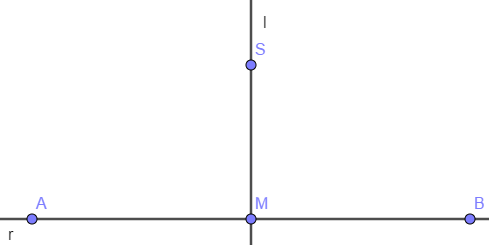
\includegraphics[width=7cm]{figuras/2-23.png}
	\vspace{-1em}
\end{figure}

\lema{2.21} Si $\sigma_r$ entonces, para todo $X$, $\m[X, \sigma_r(X)] \in r$.

\obs{2.24} Si $l \perp r$ y $g \in \iso(\P)$ entonces $g(l) \perp g(r)$.

\importante\tma{2.26} Si $l, r \subset \P$ cortan en $M$ y $\sigma_l, \sigma_r$ son dos reflexiones de $l$ y $r$, entonces se cumple que $l \perp_M r \iff r \perp_M l \iff \sigma_r(l) = l \iff \sigma_l(r) = r$.

\importante\tma{2.27 / 2.29} Para toda recta $r$ y todo punto $S \in \P - r$, existe una recta $l$ ortogonal a $r$, que pasa por $S$. Si $r$ es una recta, y $M \in r$, entonces existe $l$ tal que $l \perp_M r$.

\axioma{P7} Para toda recta $r$ y todo punto $P$ existe sólo una recta \textbf{paralela} a $r$ que pase por $P$.

\tma{2.31 / 2.33} Si $a \perp l$ y $b \perp l$ entonces $a \parallel b$. Sean $a \parallel b$. Entonces, para todo $A \in a$, la única recta $l \perp_A a$ también es ortogonal a $b$.

\tma{2.32} Las rectas parallelas forman una relación de equivalencia.
\begin{itemizex}
	\item Reflexividad: $a\parallel a$
	\item Simetría: $a \parallel b \rightarrow b \parallel a$
	\item Transitividad  $a \parallel b $ y  $b \parallel c \rightarrow a \parallel c$
\end{itemizex}

\ej{2.6} Sean $A,B \in r$, $A \neq B$. Para todo $t$, existe un único $P_t\in r$ que cumple $d(P_t,A) = \abs{t}$ y $d(P_t, B) = \abs{t-d(A,B)}$. En definitiva, la posición de $P_t$ está sólamente determinada por las distancias $d(A, P_t)$ y $d(P_t, B)$.
	 
	 
	 
	 
	 
	 
	 \end{multicols*}\pagebreak
% multicols* obliga a terminar una columna antes de empezar la siguiente.
\DeclareMathAlphabet{\pazocal}{OMS}{zplm}{m}{n}
\let\mathcal\pazocal
\usepackage{fancyhdr}
\pagestyle{fancy}
\lhead{Alex Martínez Ascensión}
\chead{}
\rhead{\today}
\date{}
\title{\Huge\vspace{-1em}Variable compleja}
\hypersetup{
 pdfauthor={},
 pdftitle={\Huge\vspace{-1em}Variable compleja},
 pdfkeywords={},
 pdfsubject={},
 pdfcreator={Emacs 26.2 (Org mode 9.2.5)}, 
 pdflang={English}}
\begin{document}

\maketitle
\vspace{-8em}

\section*{Los números complejos}
\label{sec:orga7d5865}
\begin{multicols*}{2}

\defi{1.1} Un número complejo es una expresión \(a + bi\) donde 
\(a,b \in \mathbb{R}\) y \(i\) es la unidad imaginaria, fruto de resolver la
ecuación \(x^2 + 1 = 0\) en \(\mathbb{R}\). Así, definimos \(i = \sqrt{-1}\). Si \(z \in \mathbb{C} = a + bi\), \(a = \text{Re }z\) y \(b = \text{Im
}z\) son la parte \textbf{real} e \textbf{imaginaria} de \(z\).

\defi{1.2} La \textbf{suma} y \textbf{multiplicación} están definidas en los complejos así:
\[ \left(x_{1}+y_{1} i\right)+\left(x_{2}+y_{2}
i\right)=\left(x_{1}+x_{2}\right)+\left(y_{1}+y_{2}\right) i \]
$$
\left(x_{1}+y_{1} i\right)\left(x_{2}+y_{2} i\right)=\left(x_{1} x_{2}-y_{1} y_{2}\right)+\left(x_{1} y_{2}+x_{2} y_{1}\right) i
$$
Y con estas operaciones \((\mathbb{C}, +, \cdot)\) es un cuerpo, con \(0_{\mathbb{C}} = 0 + 0i\) y \(1_\mathbb{C} = 1 + 0i\).

\defi{1.3} Dado un complejo \(z = x + yi\), llamamos \textbf{conjugado} de \(z\), \(\oveline{z}\) a \(x - yi\).

\propo{1.3.1} Se verifica que \(\overline{z_{1}+z_{2}}=\overline{z_{1}}+\overline{z_{2}}\) 
y \(\overline{z_{1} z_{2}}=\overline{z_{1}} \cdot \overline{z_{2}}\).

\defi{1.4.1} Se denomina \textbf{módulo} de un complejo \(z = x + yi\), \(|z|\) a \(\sqrt{x^2 + y^2}\). Se cumple que \(|z| = \sqrt{z\overline{z}}\). 
El módulo cumple que (1) \(|z| \ge 0\), (2) \(|z| = 0 \iff z = 0\),
(3) \(|z_1z_2| = |z_1||z_2|\) y (4) \(|z_1 + z_2| \le |z_1| + |z_2|\)

\dem{ (4) \( 
\left|z_{1}+z_{2}\right|^{2}=\left(z_{1}+z_{2}\right)(\overline{z_{1}+z_{2}})=\left(z_{1}+z_{2}\right
)(\overline{z_{1}}+\overline{z_{2}}) 
=z_{1} \overline{z_{1}}+z_{1} \overline{z_{2}}+z_{2} \overline{z_{1}}+z_{2} \overline{z_{2}} 
=z_{1} \overline{z_{1}}+z_{1} \overline{z_{2}}+\overline{z_{1} \overline{z_{2}}}+z_{2} \overline{z_{2}} 
=\left|z_{1}\right|^{2}+\left|z_{2}\right|^{2}+2 \operatorname{Re}\left(z_{1} \overline{z_{2}}\right) 
 \leq\left|z_{1}\right|^{2}+\left|z_{2}\right|^{2}+2\left|z_{1}\right|\left|z_{2}\right| 
=\left(\left|z_{1}\right|+\left|z_{2}\right|\right)^{2}
 \)  }

\defi{1.5} Dado un \(z = a + bi\), aplicando \(u = p + iq = z/|z|\),
entonces \(|u| = 1 = p^2 + q^2\). El ángulo tal que \(p = \cos \alpha, q =
\sin \alpha\) se denomina \textbf{argumento}, \(\arg z\).  Así, \(z\) puede representarse como \(z
= |z|(\cos  \alpha  + i \sin \alpha )\). Esta forma es la \textbf{forma polar}, y
también se representa como \(z = |z|e^{i\alpha}\).x 

El argumento cumple que (1) \(\arg \overline{z} = - \arg z\) y (2) \(\arg
z_1z_2 = \arg z_1 + \arg z_2\).

\defi{1.7 / 1.8} El espacio topológico \((\mathbb{C}, \delta_E)\) con distancia
euclídea no es compacto. Sin embargo, si tomamos \(\hat{\mathbb{C}} =
\mathbb{C} \cup \{ \infty \}\) entonces sí es compacto, y lo denominamos \textbf{plano
complejo ampliado}. La \textbf{esfera de Riemann}, \(\mathbb{S}\), es la representación del conjunto \(\hat{\mathbb{C}}\) en \(\mathbb{R}^3_{(\xi, \eta, \zeta)}\) en una esfera con
centro \((0, 0, 1/2)\) con ecuación \(\xi^{2}+\eta^{2}+\zeta^{2}-\zeta=0\).
\begin{figure}[H]
\centering
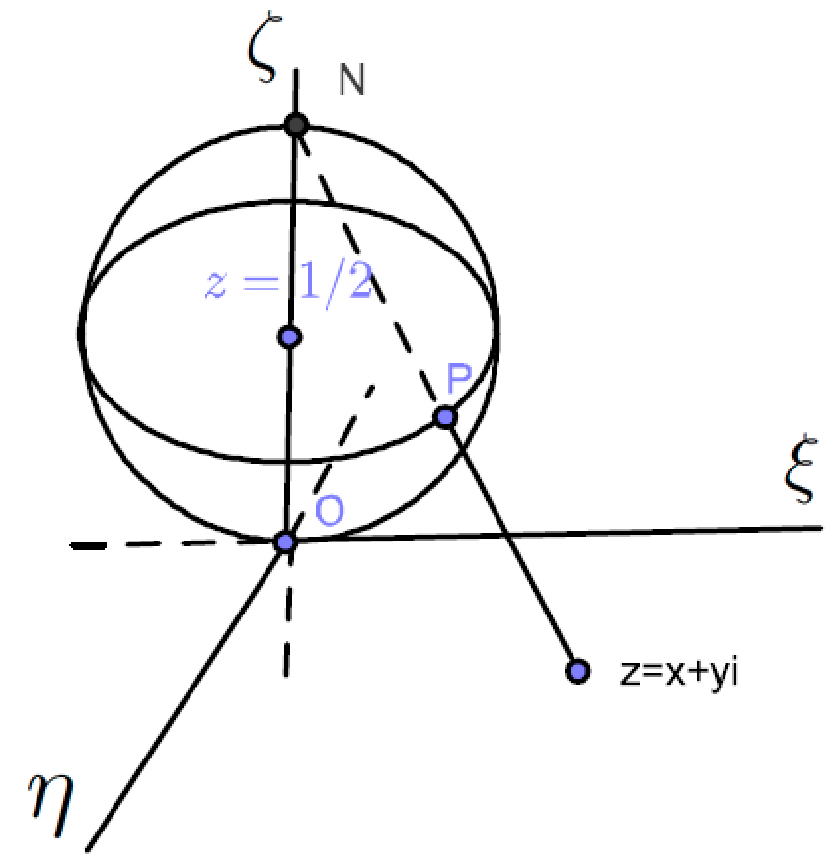
\includegraphics[width=5cm]{imagenes/esfera.png}
\end{figure}
La relación entre la esfera y el plano es 
\[ \xi=\frac{x}{1+x^{2}+y^{2}}, \eta=\frac{y}{1+x^{2}+y^{2}}, \zeta=\frac{x^{2}+y^{2}}{1+x^{2}+y^{2}} \]
La \textbf{distancia cordal} entre dos puntos \(z_1,z_2\) es la distancia euclídea 
entre los puntos \(P_1,P_2\) de la esfera de la esfera de Riemman.

\(\delta(z_1,z_2) =
 \sqrt{\left(\xi_{1}-\xi_{2}\right)^{2}+\left(\eta_{1}-\eta_{2}\right)^{2}+\left(\zeta_{1}-\zeta_{2}\right)^{2}}
 = \frac{\sqrt{\left(x_{1}-x_{2}\right)^{2}+\left(y_{1}-y_{2}\right)^{2}}}{
\sqrt{\left(1+x_{1}^{2}+y_{1}^{2}\right)\left(1+x_{2}^{2}+y_{2}^{2}\right)}}\)

Para un punto en el infinito, la distancia es \(\delta(z, \infty)=\frac{1}{\sqrt{1+x^{2}+y^{2}}}\)

\end{multicols*}
\pagebreak




\section*{Funciones complejas}
\label{sec:orgc42daf5}
\begin{multicols*}{2}
\defi{2.0} Una función puede ser de tipo \(f: \mathbb{R} \rightarrow
\mathbb{C}\) (f. compleja de var. real) o 
\(f: \mathbb{C} \rightarrow  \mathbb{C}\) (f. compleja de var. compleja).

\defi{2.1.1} \(f = f(z)\) es \textbf{continua} en \(z_0 \in \mathbb{C}\) si para todo \(\epsilon > 0\) existe \(\delta > 0\) tal que si \(|z - z_0| < \delta\)
entonces \(|f(z) - f(z_0)| < \epsilon\). \(f\) es \textbf{uniformemente continua} en
\(B \subset \mathbb{C}\) si
dado \(\epsilon > 0\) existe \(\delta > 0\) tal que para todo \(z_0 \in B\) y para todo \(z\) tal que \(|z-z_0| < \delta\) entonces \(|f(z) -
f(z_0)| < \epsilon\).  Si \(f\) es uniformemente continua es continua, pero
no siempre a la inversa.

\tma{2.1.1} Si \(f_1(z), f_2(z)\) están definidas en \(A \subset \mathbb{C}\), \(A\) abierto, y son continuas en \(z_0 \in A\), f\textsubscript{1} + f\textsubscript{2} y f\textsubscript{1}/f\textsubscript{2} son
continuas en \(z_0\). Así, los polinomios complejos son continuos.

\defi{2.1.2} Una función \(f(z)\) en \(A \subset \mathb{S}\) es continua en
\(z_0\) si para todo \(\epsilon > 0\)
 existe \(\eta > 0\) tal que para todo \(z \in A\) donde \(\delta(z, z_0) <
\eta\) entonces \(\delta(f(z_0), f(z)) < \epsilon\).

\defi{2.2.1, 2.2.2} Una función \(f(z)\) es \textbf{derivable} en \(z_0\) si existe el
límite \(\lim_{z \to z_0} \frac{f(z) - f(z_0)}{z-z_0}\) y es finito.
Si \(z_0 = \infty\), consideramos \(g(z) = f(1/z)\) y \(f\) es derivable
en \(\infty\) si \(g\) es derivable en \(z=0\).
Una función \(f:A \subset \mathbb{C} \rightarrow  \mathbb{C}\) derivable en todo
\(A\) se llama función \textbf{holomorfa} o \textbf{analítica.}

\propo{2.3.2} Si \(f\) es derivable en un punto, también es continua en ese
punto.

\propo{2.3.4 (Regla de la cadena)} Sean \(g:A \rightarrow  \mathbb{C}\) y \(f: B \rightarrow \mathbb{C}\) tales que \(g(A) \subset B\). Si \(g\) es
derivable en \(z_0\) y \(f\) es derivable en \(g(z_0)\) entonces \(f
\circ g'(z_0) = f'(g(z_0))g'(z_0)\).

\defi{2.4.1} Una función \(f: A \rightarrow  \mathbb{C}\) es conforme en \(z_0\) si existe exsite \(\theta \in [0, 2\pi]\) tal que cualquier curva \(\gamma(t)\) diferenciable en \(t_0\), \(\gamma(t_0) = z_0\) y \(\gamma'(t_0) \neq 0\) se transforma por \(f\) en una curva \(\sigma(t) =
f(\gamma(t))\) diferenciable en \(t_0\) tal que \(\sigma'(t_0) =
\gamma'(t_0) + \theta\). Si \(\alpha\) es el ángulo en el punto de cruce \(z_0\) entre \(\gamma_1, \gamma_2\), entonces el ángulo de \(f(\gamma_1),
f(\gamma_2)\) es \(\alpha\).  

\tma{2.4.1} Si \(f\) es derivable en \(z_0\) y \(f'(z_0) \neq 0\) entonces
\(f\) es conforme en \(z_0\) y \(\theta = \arg f'(z_0)\). Si \(f\) es
holomorfa, es conforme.
\dem{ Por la regla de la cadena, \( \sigma'(t_0) = f'(\gamma(t_0))\cdot \gamma'(t_0) \)  y \( \arg  \sigma'(t_0)
 = \arg f'(\gamma(t_0))+\arg  \gamma'(t_0) \) }

\defi{2.5.1} Una función de variable compleja puede transformarse a una función
\(f: \mathbb{R}^2 \rightarrow  \mathbb{R}^2\): \(f(x,y) = (u(x,y) + v(x,y)) =
u(x,y) + v(x,y)i\)

\tma{2.5.1 (Ecuaciones de Cauchy-Riemman) } Sea \(f\). \(f'(z_0)\) existe sii \(f\) es diferenciable como
función de dos variables y las funciones \(u(x,y), v(x,y)\) satisfacen
\vspace{-1em} \[
\frac{\partial u}{\partial x} = \frac{\partial v}{\partial y}, 
\frac{\partial u}{\partial y} = - \frac{\partial v}{\partial x} \]
\dem{ Suponemos \( f \) derivable en \( z_0 \) complejo, con derivada \( \lambda = f'(z_0) \). 
Si tomamos la aplicación lineal \( l_c : \mathbb{C} \rightarrow  \mathbb{C}; \eta \rightarrow \lambda\eta \).
Entonces \( \lim_{\eta \to 0} \left|\frac{f(z_0 + \eta) - f(z_0)}{\eta} - \lambda  \right| = \lim_{\eta \to 0} 
\frac{|f(z_0 + \eta) - f(z_0) - l_c(\eta)|}{|\eta|} =  0 \). Escribiendo \( f(z_0) \) y 
\( l_c(\eta) \) como componentes reales: (1) \( f(z_0) = u(x_0, y_0) + v(x_0,y_0)i = 
(u(x_0, y_0), v(x_0, y_0)) \) su jacobiano es \( D= \begin{bmatrix}
\frac{\partial u}{\partial x} &  \frac{\partial u}{\partial y} \\ 
\frac{\partial v}{\partial x} &  \frac{\partial v}{\partial y} \\ 
\end{bmatrix}  \) y (2)
\(l_c(\eta) = \lambda\eta = (\lambda_1 + \lambda_2i)(\eta_1 + \eta_2i) = (\lambda_1\eta_1 - \lambda_2\eta_2, \lambda_1\eta_2 + \lambda_2\eta_1)  \), 
que como aplicación lineal \( \mathbb{R}^2 \rightarrow  \mathbb{R}^2 \) 
es \( A= \begin{bmatrix}
\lambda_1 &  -\lambda_2 \\ 
\lambda_2 &  \lambda_1 \\ 
\end{bmatrix}  \). Como el jacobiano la derivada de \( f \) en los reales, y \( A \) es también la diferencial de 
\( f \) en \( z_0 \), \( D = A \), y se dan las ecuaciones. }

\tma{2.6.1 (Teorema de la función inversa)} Sea \(f\) analítica con derivada
continua en \(A\). Sea \(z_0 \in A\) tal que \(f'(z_0) \neq 0\). Entonces,
existen \(U, V\) abiertos tal que \(z_0 \in U\), \(f(z_0) \in V\) y \(f:
U \rightarrow  V\) es biyectiva. Además, \(f^{-1}\) es analítica en \(V\) y para
todo \(z \in U\), \((f^{-1})'(f(z)) = \frac{1}{f'(z)}\).



\end{multicols*}
\pagebreak

\section*{Series de potencias. Funciones elementales}
\label{sec:orgc694624}

\begin{multicols*}{2}

\defi{3.0.1} Una \textbf{sucesión} de complejos es una aplicación \(\mathbb{N}
\rightarrow  \mathbb{C}\) tal que para cada \(n \in \mathbb{N}\) se le
corresponde \(a_n \in \mathbb{C}\). 

\defi{3.0.2} Una \textbf{serie} es una sucesión de complejos \(\{A_n\}_{n \in \mathbb{N} }\) tal que \(A_n = \sum _{i=0}^{n} a_i\).

\defi{3.0.3} Una sucesión es de \textbf{Cauchy} o \textbf{fundamental} si dado \(\epsilon > 0\)
existe \(n_0 \in \mathbb{N}\) tal que para todo \(n_1, n_2 \ge n_0\), se
tiene que \(|a_{n_1} - a_{n_2}| < \epsilon\).

\defi{3.0.4} Se dice que \(\{a_n\}_{n \in \mathbb{N}}\) es \textbf{convergente} a \(a\)
si dado \(\epsilon > 0\) existe \(n_0 \in \mathbb{N}\) tal que para todo \(n \ge n_0\) se tiene \(|a_n-a| < \epsilon\), y diremos \(\lim_{n \to \infty}
a_n=a\).  Asimismo, \(A_n\) es convergente a \(A\) si \(\lim_{n \to \infty}
A_n = A\).

\defi{3.0.5} Una serie \(A_n\) es absolutamente convergente si la serie \(\sum |a_n|\) es convergente.

\tma{3.1.1 (Criterio de la raíz) } Dado \(\sum _{i=1}^{\infty} a_i\), sea \(\lambda = \lim_{n \to \infty} \text{sup} \sqrt[\leftroot{1}\uproot{1}n]{|a_n|}\). Si \(\lambda < 1\) la serie converge y si \(\lambda > 1\) diverge.

\tma{3.1.2 (Criterio del cociente)} Dado  
\(\sum _{i=1}^{\infty} a_i\) sea \(\beta = \lim_{n \to \infty}
\frac{|a_n|}{|a_{n-1}|}\), si \(\beta < 1\) la serie converge, y si \(\beta >
1\) diverge.

\defi{3.2.0} Una \textbf{sucesión} \textbf{de variable compleja} es una aplicación de tal manera
que a cada \(n \in \mathbb{N}\) le corresponde una función \(f_n: A
\rightarrow  \mathbb{C}\). Representamos la sucesión por \(\{ f_n \}_{n \in
\mathbb{N}}\). Asimismo, una \textbf{serie de funciones de variable compleja} es el
resultado de sumar dichas funciones: \(F_n(z) = \sum _{i=1}^{n}f_i\).

\defi{3.2.1} Una sucesión \(\{ f_n \}_{n \in N}\) converge en \(z_0 \in A\) cuando
converge la sucesión numérica \(\{ f_n(z_0) \}_{n \in \mathbb{N}}\). Diremos
que \(\{ f_n \}_{n \in \mathbb{N}}\) \textbf{converge puntualmente} cuando converge
para todo \(z \in A\).

\defi{3.2.2} La serie \(f_0 + \cdots + f_n + \cdots\) converge en un punto \(z_0 \in A\), \(A\) abierto en \(\mathbb{C}\) si la sucesión \(\{ F_n(z_0) \}_{n
\in \mathbb{N}}\) con \(F_n = f_0 + \cdots + f_n\)
converge. La serie converge puntualmente en \(A\) si \(\{ F_n \}_{n \in
\mathbb{N}}\) converge puntualmente en \(A\).

\defi{3.2.3} La sucesión de funciones \(\{ f_n \}_{n \in N}\) converge
uniformemente a \(f\) si para todo \(\epsilon > 0\) existe \(n_0 \in
\mathbb{N}\) tal que \(|f_n(z) - f(z)| < \epsilon\) para todo \(z \in A, n
\ge n_0\). 

\defi{3.2.4} La serie \(\sum _{n=1}^{\infty} f_n(z)\) converge uniformemente
en \(A\) si la sucesión \(\{ F_n \}_{n \in N}\) converge uniformemente en \(A\).

\tma{3.2.1 Criterio de la mayorante de Weierstrass)} Una condición suficiente
para que \(\sum _{n=1}^{\infty} f_n\) converja uniformemente en \(A \subset
\mathbb{C}\) es que exista una serie \(\sum _{n=1}^{\infty} a_n\) convergente
tal que \(|f_n(z)| \le a_n\) para todo \(z\) y \(n \in \mathbb{N}\).
En tal caso, \(\sum _{n=1}^{\infty} a_n\) es una mayorante de \(\sum
_{n=1}^{\infty} f_n\). 

\defi{3.3.0} Una \textbf{serie de potencias} es una serie de la forma \(\sum
_{n=1}^{\infty} a_n(z - z_0)^n\), con \(z_0, a_n \in \mathbb{C}\) para todo
\(n\). Los \(a_n\) se llaman \textbf{coeficientes} de la serie.
Si \(z_0=0\), es decir, \(\sum _{n=1}^{\infty} a_nz^n\) decimos que la serie
está \textbf{centrada en el origen}.

\defi{3.3.1 (Teorema de Cauchy-Hadamard)} Dada la serie \(\sum _{n=1}^{\infty}
a_n(z - z_0)^n\) considerando  \(\lambda = \lim_{n \to \infty} \text{sup} \sqrt[\leftroot{1}\uproot{1}n]{|a_n|}\); si llamamos \(R = \frac{1}{\lambda}\), tenemos:
\begin{itemize}
\item La serie converge absolutamente en el interior del círculo \(D_R = \{z| |z-z_0| < R \}\) y diverge en el exterior \(\overline{D_R} = \{ z| |z-z_0|> R \}\)
\item La convergencia es uniforme en todo circulo de radio \(0 \le r < R\)
\end{itemize}
\(R\) se llama \textbf{radio de convergencia} de la serie. 


\tma{3.3.2} La función definida por la suma de serie de potencias en su círculo
de convergencia es derivable en todo punto de dicho círculo:
\[ \frac{\text{d}}{\text{d}z} \left( \sum _{n=0}^{\infty}a_n(z-z_0)^n \right) = 
\sum _{n=0}^{\infty}na_n(z-z_0)^{n-1} \].

\defi{3.4.1} La función exponencial compleja es \[ e^z = \sum_{n=0}^{\infty}
\frac{z^n}{n!} \].
Su radio de convergencia es \(R = \infty\). Cumple también que \(e^{z_1+z_2}
 = e^{z_1}e^{z_2}\).
El exponente puede reescribirse como \(e^z = e^{x+yi} = e^xe^{iy} = e^x(\cos
y + i \sin y)\)

\defi{3.4.2} La función logaritmo se obtiene desde la exponencial. Escribiendo
\(z = r e^{i\theta}\) tenemos que \(\log z  = \log|r| + i\theta = \log|r| + i
\arg(z)\). Como \(\arg(z) = \theta + 2\pi k\), el logaritmo principal es \(\theta \in [0, 2\pi] = \text{Arg } z\).

\defi{3.4.3} Las funciones seno y coseno se definen a través de sus series de
potencias con \(R = \infty\):
\[ \sin(z) = \sum _{n=0}^{\infty} (-1)^n \frac{z^{2n+1}}{(2n+1)!}\;,\; 
\cos(z) = \sum _{n=0}^{\infty}(-1)^n \frac{z^{2n}}{(2n)!} \]
La derivación es como con los números reales, y las identidades de Euler son
idénticas:
\[ \cos(z) = \frac{e^{iz} + e^{-iz}}{2} \;,\; \sin(z) = \frac{e^{iz} -
e^{-iz}}{2i} \]
\[ \sinh(z) = \frac{e^z - e^{-z}}{2}\;,\; \cosh(z) = \frac{e^z + e^{-z}}{2} \]

\defi{3.4.4} La función potencial con exponente complejo, \(z^\zeta, \zeta \in
\mathbb{C}\) es \(z^{\zeta} = e^{\zeta \log z}\)

\defi{3.5.1 (Funciones multiformes)}  Una función \(f\) es multiforme cuando
\(w = f(z)\) puede tomar diferentes valores para el mismo \(z\). Por
ejemplo, para \(f = \sqrt{z}\), \(f(2i) = 1+i\) y \(f(2i) = -1-i\). 
Esto se debe a que \(z^{1/2} = e^{\frac{1}{2} \log{z}} =
e^{\frac{1}{2}(\log{|z| + i \arg(z))}} = |z|^{\frac{1}{2}}e^{i \frac{\text{Arg
}z + 2k\pi}{2}}, k = 0,1\).

Observamos que como \(k\) puede tomar dos valores, entonces la función tiene
dos ramas, es decir, \(w_1 = \sqrt{r}e^{i \frac{\theta}{2}}\;,\;w_2 =
-\sqrt{r}e^{-i \frac{\theta}{2}}\).
Por tanto, para completar un ciclo en \(w\) necesitamos completar dos ciclos
en \(z\) (uno por rama). Esto genera una \textbf{superficie de Riemann} como la
siguiente figura:

\begin{figure}[H]
\centering
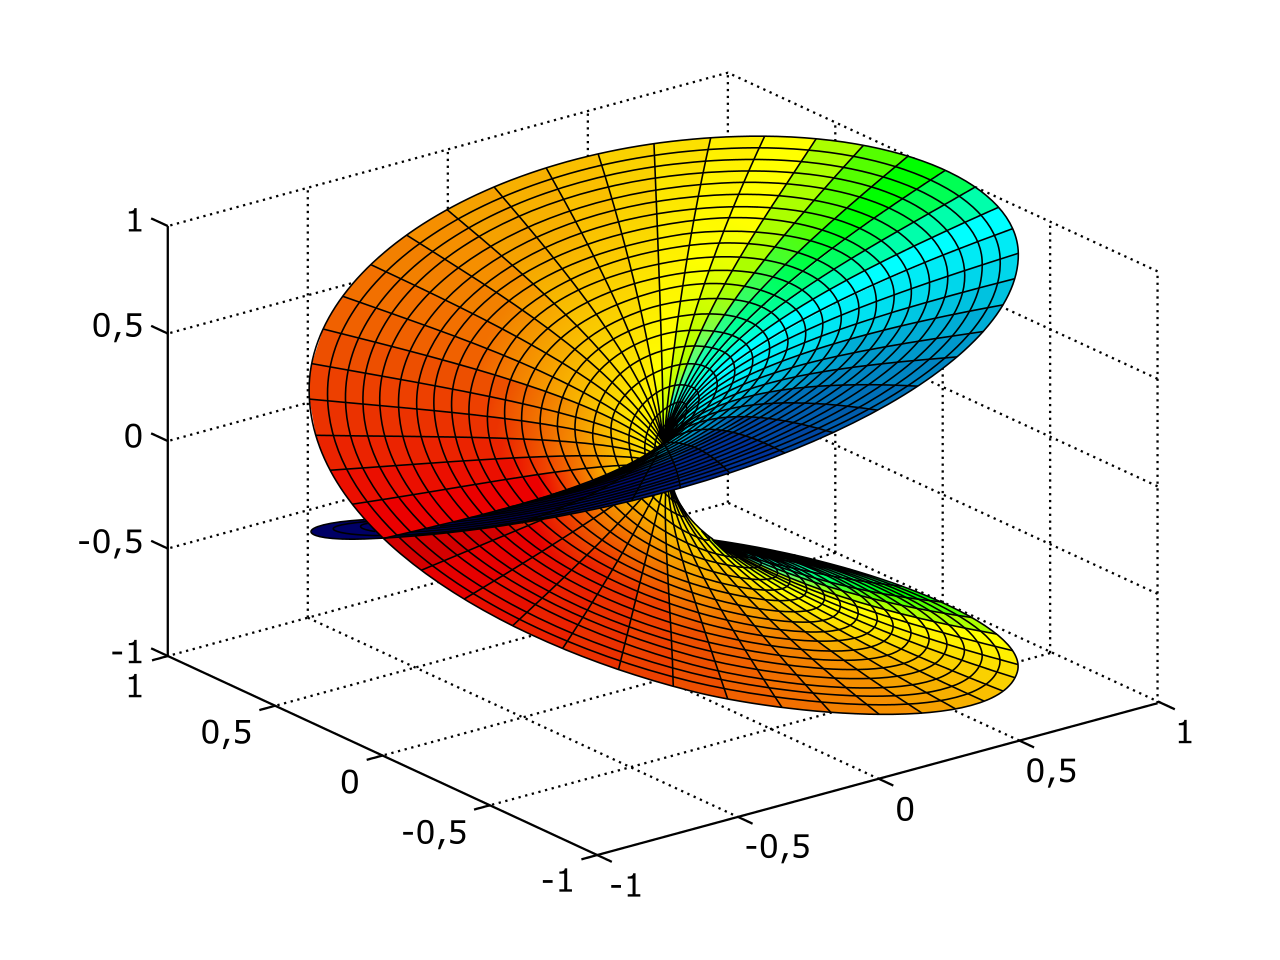
\includegraphics[width=9cm]{imagenes/riemann_sqrt.png}
\end{figure}

En este caso los ejes \(X\) e \(Y\) representan el plano complejo de \(z\). El eje \(Z\) representa la parte real de \(f(z)\), y el color representa
la imaginaria. El punto de corte del plano es el caso \(\sqrt{-a}, a \in
\mathbb{R}  = 0 + i \sqrt{a}\). Sin embargo, el corte es un artefacto de la
visualización tridimensional de 4 dimensiones.

Debajo se muestra el ejemplo de \(f = \log{z}\), donde el eje \(X\)
representa el argumento, y el color representa la parte real. 

\begin{figure}[H]
\centering
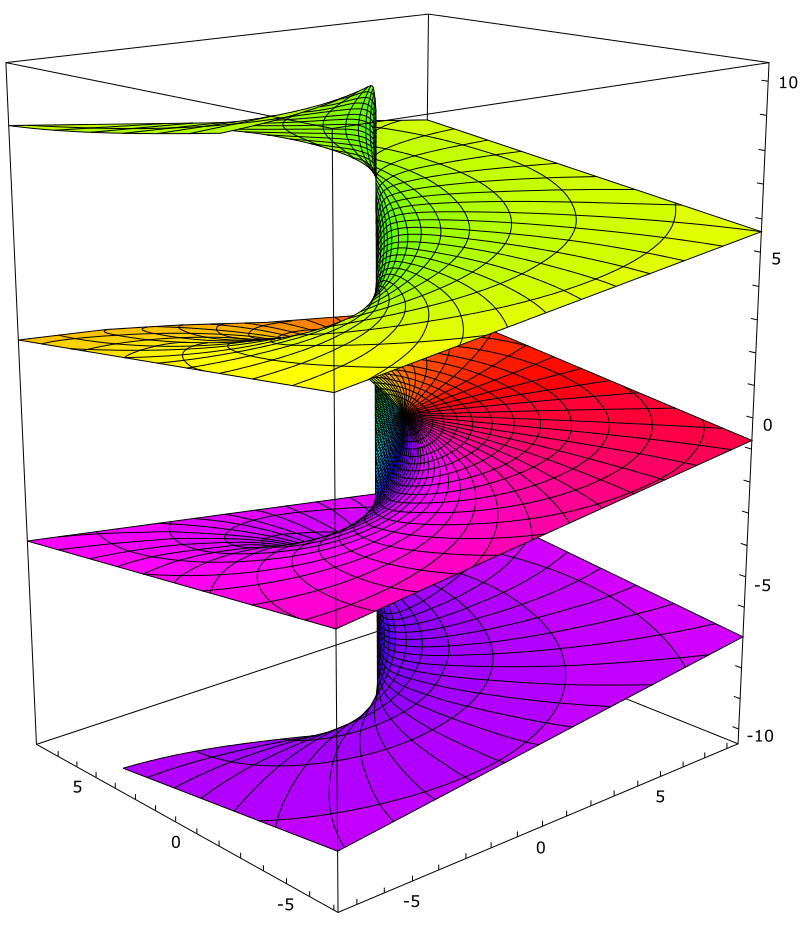
\includegraphics[width=8cm]{imagenes/riemann_log.png}
\end{figure}

Vemos que el el plano "cae" de nivel en cada vuelta. Esto es el equivalente a
cada rama del logaritmo.


\end{multicols*}
\pagebreak

\section*{Integración en el campo complejo}
\label{sec:org74cd684}
\begin{multicols*}{2}


\defi{4.0.1} Una curva \(\gamma:[a,b] \rightarrow  \mathbb{C}\) es
\textbf{rectificable} cuando presenta una longitud finita.

\defi{4.0.2} Una \textbf{partición} de un intervalo es el conjunto \(\Delta = \{ a =
t_0 < t_1 < \cdots < t_n = b \}\). La \textbf{norma} de la partición es \(|\Delta| =
\max \{ |t_{k-1} - t_k|, k = 0, 1, \cdots, n-1 \}\). Una partición \(\Delta'\) es \textbf{más fina} que otra partición \(\Delta\) cuando \(\Delta \subset \Delta'\).

\defi{4.0.3} Dados \(f, \gamma, \Delta\), definimos la suma de
Riemman-Stieljes como \(S(\Delta, f, \gamma) = \sum_{k=0}^{n-1}
f(s_k)[\gamma(t_{k+1}) - \gamma(t_{k})]\), con \(s_k \in [t_k, t_{k+1}]\).
\(f\) es \textbf{integrable} Riemman-Stieljes (RS) si existe un complejo \(I\) tal que 
para cualquier \(\epsilon > 0\)
existe una partición \(\Delta_{\epsilon}\) tal que para toda \(\Delta_{\epsilon} \subset \Delta\), \(|S(\Delta, f, \gamma) - I| < \epsilon\). \(I\) se denota por \(\int_ { a }^{ b } f \; \text{d}\gamma\).

\defi{4.0.4} Si \(\gamma(t) = \phi(t) + i \psi(t)\), entonces \(\int_ { a }^{ b } f \;
 \text{d}\gamma 
 = \int_ { a }^{ b } f \; \text{d}\phi + i \int_ { a }^{ b } f \; \text{d}\psi\).

\propo{4.1.1} Sean \(f, \gamma\). Entonces existe la integral RS y 
\(\left|\int_ { a }^{ b } f \; \text{d}\gamma  \right| \le ML(\gamma)\), 
donde \(M = \max \{ |f(t)|\;|\;t \in [a,b] \}\) y \(L(\gamma)\) es la
longitud de \(\gamma\).
\dem{ \( |S(\Delta, f, \gamma)|  \leq \sum_{k=0}^{n-1}\left|f\left(s_{k}\right)\right|\left|\gamma\left(t_{k+1}\right)-\gamma\left(t_{k}\right)\right| 
 \leq(\max \{|f(t)|, t \in[a, b]\}) \sum_{k=0}^{n-1}\left|\gamma\left(t_{k+1}\right)-\gamma\left(t_{k}\right)\right| 
 \leq M L(\gamma)\) }

\propo{4.1.2} Si \(f\) es continua en \([a, b]\) y \(\gamma\) define un
camino de clase \(C^1\) entonces la integral RS viene dada por 
\(\int_{a}^{b} f \text{d} \gamma=\int_{a}^{b} f \gamma^{\prime} \text{d} t\)
\dem{ Como \( \int_ { a }^{ b } f \;
 \text{d}\gamma 
 = \int_ { a }^{ b } f \; \text{d}\phi + i \int_ { a }^{ b } f \; \text{d}\psi   \), vamos a demostrar que 
\( \int_ { a }^{ b } f \; \text{d}\phi = \int_ { a }^{ b } f \phi'\; \text{d}t \).
Por la definición de \( I \) existe para todo \( \epsilon > 0 \) una partición tal que \( 
 \left|\sum_{k=0}^{n-1} f\left(s_{k}\right)\left[\varphi\left(t_{k+1}\right)-\varphi\left(t_{k}\right)\right]-\int_{a}^{b} f d \varphi\right|<\epsilon \) 
Por el teorema del valor intermedio: \( \varphi\left(t_{k+1}\right)-\varphi\left(t_{k}\right)=\varphi^{\prime}\left(s_{k}^{\prime}\right)\left(t_{k+1}-t_{k}\right) \),
luego \(  |\sum_{k=0}^{n-1} f\left(s_{k}^{\prime}\right) \varphi^{\prime}\left(s_{k}^{\prime}\right)\left(t_{k+1}-t_{k}\right)-\int_{a}^{b} f d \varphi|<\epsilon\).
Ahora bien, la expresión de sumatorio puede aplicarse a la integral, de modo que 
\(|\sum_{k=0}^{n-1} f\left(s_{k}^{\prime}\right) \varphi^{\prime}\left(s_{k}^{\prime}\right)\left(t_{k+1}-t_{k}\right)-\int_{a}^{b} f \varphi^{\prime} d t|<\epsilon \).
Por último, si denominamos \( S \) al sumatorio anterior, tenemos que \( |\int_{a}^{b} f \varphi^{\prime} d t - 
\int_{a}^{b} f d \varphi | \le |\int_{a}^{b} f \varphi^{\prime} d t - S| + | S - \int_{a}^{b} f d \varphi | \le 2 \epsilon \). 
Repetimos para \( \int_ { a }^{ b } f \; \text{d}\psi  \) y finalmente 
\(  \int_ { a }^{ b } f \; \text{d}\gamma =  \int_ { a }^{ b } f \; \text{d}\phi + i  \int_ { a }^{ b } f \; \text{d}\psi 
=  \int_ { a }^{ b } f\phi' \; \text{d}t + i  \int_ { a }^{ b } f\psi' \; \text{d}t =  
\int_ { a }^{ b } f\gamma' \; \text{d}t \)}

\defi{4.2.0} Sean \(f, \gamma\). Se define la \textbf{integral de \(f\) a lo largo
de \(\gamma\)}, \(\int_\gamma fdz\) como \(\int_ { a }^{ b } f \circ \gamma
\; \text{d}\gamma\) y, si \(\gamma\) es \(C^1\), entonces \(\int_\gamma
fdz = \int_ { a }^{ b } f(\gamma(t))\gamma'(t)  \; \text{d} t\).
La integral cumple:
\begin{itemize}
\item Linealidad: \(\int _\gamma (c_1f_1 + c_2f_2) \; \text{d}z  = c_1 \int _\gamma
  f_1\; \text{d} z + c_2 \int _\gamma f_2 \; \text{d}z\)
\item Si \(-\gamma\) es el camino opuesto a \(\gamma\): \(\int _\gamma f \;
  \text{d}z = - \int _{-\gamma} f \; \text{d}z\)
\item Yuxtaposición: \(\int _{\gamma_1 \cup \gamma_2} f \; \text{d}z = \int
  _{\gamma_1} f \; \text{d}z  + \int _{\gamma_2} f \; \text{d}z\)
\item Se tiene la siguiente stimación: \(|\int _\gamma f \; \text{d}z| \le \int _\gamma |f|| \; \text{d}z|  = \int_ { a
  }^{ b } |f(t)||\gamma'(t)| \; \text{d}t  \le ML(\gamma)\).
\end{itemize}

\propo{4.2.1} Sea \(\{ f_n \}_{n \in \mathbb{N}}\) una sucesión de funciones,
y \(\gamma\). Si \(f_n\) son continuas y \(f_n \rightarrow  f\) entonces
\(\lim_{n \to \infty} \int _{\gamma} f_n = \int _\gamma f dz\). 
\dem{ Si \( |dz| \) es la longitud de la curva, \( L \), entonces \( \left|\int_{\gamma} f d z-\int_{\gamma} f_{n} d z\right| \leq \int_{\gamma}\left|f-f_{n}\right||d z|<\epsilon L \)
 }.

También, si \(\sum f_n\) converge uniformemente a \(F\), entonces \(\sum
_{n=1}^{\infty} \int _\gamma f_n \; \text{d}z  = \int _\gamma F \; \text{d}z\). 
\dem{ \(
\int_{\gamma}\left(\sum_{n=1}^{\infty} f_{n}\right) d z &=\int_{\gamma}\left(\lim _{n \rightarrow \infty} F_{n}\right) d z=\lim _{n \rightarrow \infty} \int_{\gamma} F_{n} d z 
=\lim _{n \rightarrow \infty} \int_{\gamma}\left(\sum_{k=1}^{n} f_{k}\right) d z=\lim _{n \rightarrow \infty} \sum_{k=1}^{n} \int_{\gamma} f_{k} d z=\sum_{n=1}^{\infty} \int_{\gamma} f_{n} d z
 \)  }


\propo{4.3.1} Sean \(f, \gamma\), \(\gamma: [a,b] \rightarrow  \mathbb{C}\) de clase \(\mathbb{C}^1\). Si
\(F\) es una frimitiva de \(F\), se tiene que \(\int _\gamma f \; \text{d}
z\) = F(\(\gamma\)(a)) - F(\(\gamma\)(b)).
\dem{ Si \( \int _\gamma f \; \text{d}z = \int_ { a }^{ b } f(\gamma(t))\gamma'(t) \; \text{d}t   \), como la derivada de 
\( F(\gamma(t) = F'(\gamma(t))\gamma'(t) = f(\gamma(t))\gamma'(t) \); por el Teorema Fundamental del Cálculo se cumple 
que \(\int_{\gamma} f d z =\int_{a}^{b}[F(\gamma(t))]^{\prime} d t=F(\gamma(b))-F(\gamma(a)) \)}

\propo{4.3.2} Sea \(f\) y \(\gamma_1, \gamma_2\) tales que \(\gamma_1(a) =
\gamma_2(a)\) y \(\gamma_1(b) = \gamma_2(b)\). Entonces \(\int _{\gamma_1}f
\; \text{d}z  = \int _{\gamma_2}f \; \text{d}z\).


\tma{4.4.1 (Preliminar del T de Cauchy)} Sea \(f\) analítica y \(\gamma
\subset A\) es una curva cerrada y su interior. Entonces \(\int _\gamma f \;
\text{d}z  = 0\).
\dem{ La fórmula de Green indica que \( \int_{\gamma} P(x, y) d x+Q(x, y) d y=\iint_{A}\left[\frac{\partial Q}{\partial x}(x, y)-\frac{\partial P}{\partial y}(x, y)\right] d x d y \)
Con \( A \) el interior de \( \gamma \). Si describimos \( f = u(x,y) + iv(x,y) \) operando
tenemos que 
\(\int_{\gamma} f d z =\int_{\gamma}(u+i v)(d x+i d y) 
=\int_{\gamma}(u d x-v d y)+i \int_{\gamma}(u d y+v d x)\). Applicando el teorema de Green 
tenemos que \( \int_{\gamma} f d z=\iint_{A}\left[-\frac{\partial v}{\partial x}-\frac{\partial u}{\partial y}\right] d x d y+\iint_{A}\left[\frac{\partial u}{\partial x}-\frac{\partial v}{\partial y}\right] d x d y \)
y, por las ecs. de Cauchy-Riemman, \( - \frac{\partial v}{\partial x} - \frac{\partial u}{\partial y} = 
\frac{\partial u}{\partial y} - \frac{\partial u}{\partial y} = 0\). Ídem para la segunda integral.  }

\tma{4.4.2 (T de Cauchy-Goursat para el triángulo)} Sea \(f: A \rightarrow
\mathbb{C}\), \(A \subset \mathbb{C}\) abierto, y \(f\) analítica en \(A\
\{ p \}\). Si \(T\) es el triángulo cerrado contenido en \(A\), se tiene \(\int _{\partial T} f \; \text{d} z = 0\).

\tma{4.4.3 (T de Cauchy para un conjunto convexo}. Sea \(f\) analítica en \(A\{p}\) con \(p \in A\) y continua en \(A\). Entonces   \(\int _{\partial T} f \; \text{d} z = 0\) para todo camino cerrado y
rectificable en \(A\).

\end{multicols*}
\pagebreak

\section*{Consecuencias del Teorema de Cauchy}
\label{sec:org164e837}
\begin{multicols*}{2}


\defi{5.0} Llamamos \textbf{índice} de \(\gamma\) respecto de \(\alpha\),
representado por \(Ind_{\gamma}(\alpha)\) a la integral 
\[ Ind_{\gamma}(\alpha) = \frac{1}{2\pi i}\int _\gamma \frac{\text{d}
z}{z-\alpha}   \]
Intuitivamente \(Ind_\gamma(\alpha)\) representa el número de vueltas de \(\gamma\) respecto de \(\alpha\).
\dem{ La función \( \frac{1}{z-\alpha} \) admite la primitiva \( \log{z - \alpha} \) en todo entorno expcepto 
para \( \alpha \). Subdividimos \( \gamma \) en subarcos suficientemente pequeños \( \gamma_1, \gamma_2, \cdots, \gamma_n \), tal que
\( \gamma_i = z_iz_{i+1}; z_i,z_{i+1} \in \gamma \). Así, la integral se puede calcular como 
\( \frac{1}{2\pi i} \int _\gamma  \frac{\text{d} z}{z - \alpha} =
 \sum _{j=1}^{n-1} \frac{1}{2\pi i} \int _{\gamma_j}  \frac{\text{d} z}{z - \alpha} 
= \sum_{j=1}^{n-1} \frac{1}{2 \pi i}[\ln (z_{j+1}-\alpha)-\ln (z_{j}-\alpha)] = 
 \sum_{j=1}^{n-1} \frac{1}{2 \pi i}[\ln |(z_{j+1}-\alpha)|-\ln |(z_{j}-\alpha)|]+\sum_{j=1}^{n-1} 
\frac{1}{2 \pi}[\operatorname{Arg}(z_{j+1}-\alpha)-\operatorname{Arg}(z_{j}-\alpha)]
 \). La primera suma es 0 por ser teléscopica y \( z_1 = z_n \), luego 
\( \frac{1}{2\pi i} \int _\gamma  \frac{\text{d} z}{z - \alpha} = \sum_{j=1}^{n-1} 
\frac{1}{2 \pi}[\operatorname{Arg}(z_{j+1}-\alpha)-\operatorname{Arg}(z_{j}-\alpha)] \). Cada elemento de la suma
es una variación de la circunferencia, y en conjunto representa el número de vueltas
recorrido.}

\tma{5.1.1} Si \(\gamma\) es diferenciable cerrado, \(\gamma^*\) su
interior, entonces \(Ind_\gamma(\alpha)\) es
entero si \(\alpha \in \gamma^*\), o es cero si \(\alpha \in
\mathbb{C}/\gamma^*\). 

\tma{5.2.1 (Fórmula integral de Cauchy)} Sea \(f: A \rightarrow  \mathbb{C}\),
y sea \(\gamma\) un camino cerrado en \(A\). Entonces para todo \(z \in A\) tal que \(z \not \in \gamma^*\)
 se tiene \[ f(z) Ind_\gamma(z) = \frac{1}{2\pi i}\int _\gamma
\frac{f(\zeta)}{\zeta - z} \text{d}\zeta   \]
\dem{  Definimos $g: A \rightarrow \mathbb{C}$ mediante:
$$
g(\zeta)=\left\{\begin{array}{cccc}
\frac{f(\zeta)-f(z)}{\zeta-z} & \text { para } & \zeta \in A, & \zeta \neq z \\
f^{\prime}(z) & \text { para } & \zeta=z
\end{array}\right.
$$
donde $z \in A \backslash \gamma^{*}$ es un punto fijo. La función $g$ es analítica para $\zeta \neq z$ y
$
g^{\prime}(\zeta)=\frac{(\zeta-z) f^{\prime}(\zeta)-f(\zeta)+f(z)}{(\zeta-z)^{2}}
$
y es continua para $\zeta=z$ pues
$
\lim _{\zeta \rightarrow z} g(\zeta)=f^{\prime}(z)
$.
Por tanto podemos aplicar el Teorema de Cauchy-Goursat y 
$
\frac{1}{2 \pi i} \int_{\gamma} g(\zeta) d \zeta=0
$ y como $z \notin \gamma^{*},$ se puede escribir
$
0 =\frac{1}{2 \pi i} \int_{\gamma} \frac{f(\zeta)-f(z)}{\zeta-z} d \zeta=\frac{1}{2 \pi i} \int \frac{f(\zeta)}{\zeta-z} d \zeta 
-\frac{f(z)}{2 \pi i} \int_{\gamma} \frac{d \zeta}{\zeta-z} \iff \frac{f(z)}{2 \pi i} 
\int_{\gamma} \frac{d \zeta}{\zeta-z}=\frac{1}{2 \pi i} \int_{\gamma} \frac{f(\zeta)}{\zeta-z} d \zeta
$
es decir
$f(z) \operatorname{Ind}_{\gamma}(z)=\frac{1}{2 \pi i} \int_{\gamma} \frac{f(\zeta)}{\zeta-z} d \zeta$ }

\tma{5.3.1 (Teorema de Taylor)} 
Sea \(f\) holomorfa, \(A \subset \mathbb{C}\) abierto,
y \(\alpha \in A\). Sea \(d>0\) la distancia de \(\alpha\) a la frontera de \(A\); 
entonces para todo \(z \in B(\alpha, d)\)
$$
f(z)=\sum_{n=0}^{\infty} \frac{f^{(n)}(\alpha)}{n !}(z-\alpha)^{n}
$$
El radio de convergencia es mayor o igual que
\(d\), y en \(B(\alpha, d)\) su suma es \(f(z)\). 
Además las derivadas sucesivas \(f^{(n)}\) \((\alpha)\) de \(f\) en \(\alpha\) vienen dadas por
$$
f^{(n)}(\alpha)=\frac{n !}{2 \pi i} \int_{\gamma} \frac{f(\zeta)}{(\zeta-\alpha)^{n+1}} d \zeta
$$
donde \(\gamma\) es una circunferencia de centro \(\alpha\) y radio \(r\), con
\(0<r<d\).

\tma{5.4.1 (Desigualdades de Cauchy)} Si \(f\) es analítica y \(B(\alpha, d)
\subset A\) entonces 
\(|f^{(n)}(\alpha)| \le \frac{n!M(r)}{r^n}\), con \(M(r) =
\max_{|z|=r<d}|f(z)|\)

\tma{5.4.2 (Teorema de Liouville)} Si \(f\) es entera (analítica en todo \(\mathbb{C}\)) y acotada, entonces es constante.
\dem{  Por ser $f$ analítica existe un desarrollo
$
f(z)=\sum_{n=0}^{\infty} a_{n} z^{n}
$
con radio de convergencia infinito. Sea $K$ una cota de $f$, es decir
$
|f(z)|<K, \text { para todo } z \in \mathbb{C}
$
entonces de las desigualdades de Cauchy se obtiene
$
\left|a_{n}\right|<\frac{K}{r^{n}}, n=1,2, . .
$
para todo $r$. Como \( r \rightarrow \infty \), \( a_n \rightarrow 0 \) y \( f(z) = a_0 \). }

\tma{5.5.1} Sea \(\{ f_n \}_{n \in \mathbb{N}}\) una sucesión de funciones 
analíticas en \(A\) que converge uniformemente en todo compacto de \(A\).
Entonces la sucesión \(\{ f'_n \}\) converge uniformemente en todo compacto
de \(A\). Además, si \(\lim_{n \to \infty} f_n(z) = f(z)\) entonces \(\lim_{n \to \infty} f'_n(z) = f'(z)\) para todo \(z \in A\).

\begin{figure}[H]
\centering
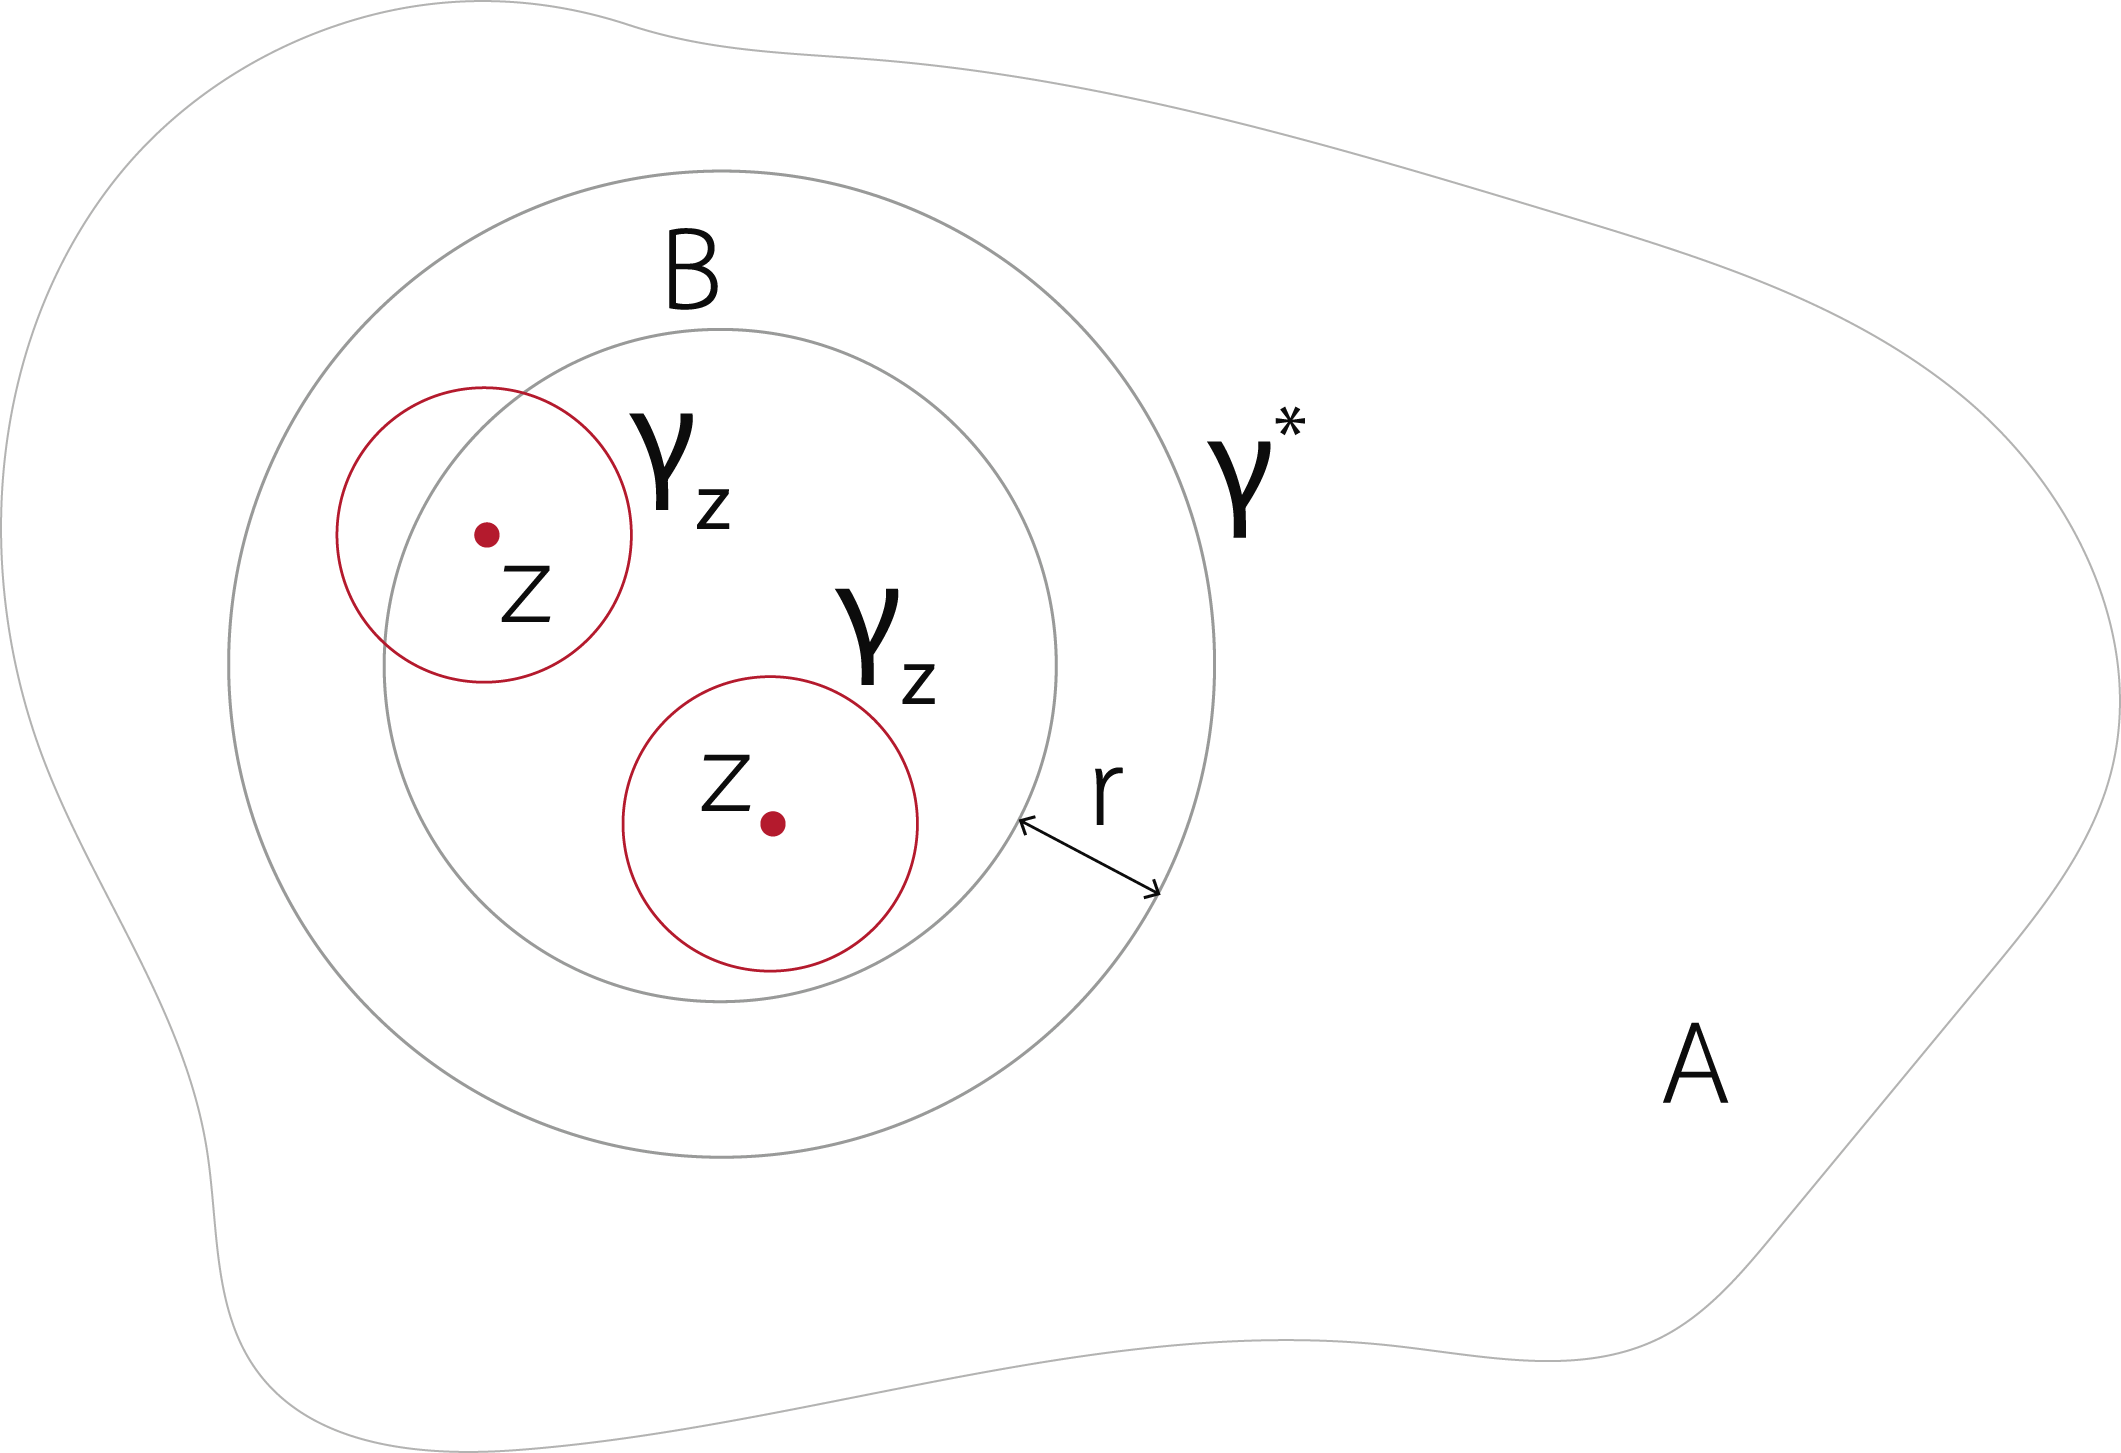
\includegraphics[width=7cm]{imagenes/T-5_5_1.png}
\end{figure}

\dem{   Bastará demostrar la convergencia uniforme de la sucesión
$\left\{f_{n}^{\prime}\right\}$ a $f^{\prime}$ en todo círculo $B \subset A,$ pues todo compacto
 $K \subset A$ puede ser recubierto por una cantidad finita de círculos.
Sea $\gamma^{*} \subset A$ una circunferencia concéntrica con $B$ con $r = r_\gamma - r_B$.
 Sea $z \in B$ y $\gamma_{z}$ la circunferencia de centro $z$ y 
radio $r$. Entonces
$
f^{\prime}(z)=\frac{1}{2 \pi i} \int_{\gamma_{z}} \frac{f(\zeta)}{(\zeta-z)^{2}} d \zeta, \quad f_{n}^{\prime}(z)
=\frac{1}{2 \pi i} \int_{\gamma_{z}} \frac{f_{n}(\zeta)}{(\zeta-z)^{2}} d \zeta
$
de donde
$
|f^{\prime}(z)-f_{n}^{\prime}(z)|  \leq \frac{1}{2 \pi} \int_{\gamma_{z}} 
\frac{eft|f(\zeta)-f_{n}(\zeta)|}{|\zeta-z|^{2}}|d \zeta|
 \leq \frac{1}{2 \pi} \frac{M_{n}}{r^{2}} 2 \pi r=\frac{M_{n}}{r}
$
donde $M_{n}$ es $\max(\left|f(\zeta)-f_{n}(\zeta)\right|)$
en $\gamma_z$.
Puesto que $\left\{f_{n}\right\}$ converge uniformemente sobre todo círculo 
cerrado, se tiene que
$
\lim _{n \rightarrow \infty} M_{n}=0
$ de tal manera que $\frac{M_{n}}{r}<\epsilon$
para $n \geq n_{0}$, y $z \in B$ .
}

\defi{5.6} \(f\) en \(A \subset \mathbb{C}\) tiene la \textbf{propiedad de la media}
si para todo cerrado \(\overline{D}(\alpha, r) = \{ z \;|\; |z - \alpha| \le r
\} \subset A\), el valor \(f(\alpha)\) en el centro es la media de f en la
circunferencia:
\[ f(\alpha) = \frac{1}{2 \pi} \int_{0}^{2 \pi} f\left(\alpha+r e^{i t}\right) d t \]

\propo{5.6.1} Toda función analítica \(f\) en \(A\) tiene la propiedad de
la media.

\tma{5.6.1 (Principio del módulo máximo)}
Sea \(f\) analítica en \(A\), abierto conexo. Entonces para todo \(\alpha
\in A\) en cualquier entorno de \(\alpha\) existe \(\beta \in A\) para el
cual \(|f(\alpha)| < |f(\beta)|\).

\lema{5.7.1 (Lema de Schwarz)}
Sea \(f: B(0,1) \rightarrow  B(0,1)\) analítica. \(|f(z)| < 1\) para todo \(z
\in B(0,1)\) y \(f(0) = 0\). Entonces se tiene \(|f(z)| \leq|z|\) para todo
 \(z \in B(0,1)\) y \(\left|f^{\prime}(0)\right| \leq 1\). 
Además, si para un \(z_{0} \in B(0,1), z_{0} \neq 0\), se tiene 
\(\left|f\left(z_{0}\right)\right|=\left|z_{0}\right|\), o si se verifica 
\(f^{\prime}(0)=1\), entonces \(f(z)\) es de la forma \(f(z)=c z\), con \(|c|=1\)

\end{multicols*}
\pagebreak
\end{document}